\chapter{Theory of drift diffusion modelling}
\label{sec:electrical}

\section{Outline}
OghmaNano's electrical model is a 1D/2D drift-diffusion model (like many others) however the special thing about OghmaNano which makes it very good for disordered materials (Think organics, perovskites and a-Si) is that it goes to the trouble of explicitly solving the Shockley-Read-Hall equations as a function of energy and position space.  This enables one to model effects such as mobility/recombination rates changing as a function of carrier population and enables one to correctly model transients as one does not have to assume all the carriers in the trap states have reached equilibrium.  Things such as ToF transients, CELIV transients etc.. can be modelled with ease. Of course can be used for more ordered materials as well, you then just need to turn the traps off.


\section{Electrostatic potential}
The conduction band/valance band (or LUMO/HOMO in organic semiconductor speak) are defined as

\begin{equation}
E_{LUMO}=-\chi-q\phi
\end{equation}

\begin{equation}
E_{HOMO}=-\chi-E_g-q\phi
\end{equation}

To obtain the internal potential distribution within the device Poisson's equation is solved,

\begin{equation}
\label{eq:pos}
\nabla \cdot \epsilon_0 \epsilon_r \nabla = q (n_{f}+n_{t}-p_{f}-p_{t}-N_{ad}+-N_{ion}+a),
\end{equation}

where $n_{f}$, $n_{t}$ are the carrier densities of free and trapped electrons; $p_{f}$ and $p_{t}$ are the carrier densities of the free and trapped holes; and $N_{ad}$ is the doping density. $N_{ion}$ is the background density of perovskite ions and a is the density of mobile ions.

\section{Free charge carrier statistics}
For free carriers the model can either use Maxwell-Boltzmann statistics i.e.

\begin{equation}
n_{l}=N_c exp \left (\frac{F_n-E_{c}}{kT} \right)
\end{equation}

\begin{equation}
p_{l}=N_v exp \left(\frac{E_{v}-F_p}{kT} \right)
\end{equation}


or full Fermi-dirac statistics i.e.

\begin{equation}
n_{free}(E_{f},T)=\int^{\infty}_{E_{min}} \rho(E) f(E,E_{f},T) dE
\end{equation}

\begin{equation}
p_{free}(E_{f},T)=\int^{\infty}_{E_{min}} \rho(E) f(E,E_{f},T) dE
\end{equation}

where

\begin{equation}
f(E)=\frac{1}{1+e^{{E-E_f}/kT}}
\end{equation}

When using FD statistics free carriers are assumed to move in a parabolic band:

\begin{equation}
\rho(E)_{3D}=\frac{\sqrt{E}}{4\pi^2} \left ( \frac{2m^{*}}{\hbar^2}\right )^{3/2}
\end{equation}

The average energy of the carriers is defined as

\begin{equation}
\label{eq:energy}
\bar{W}(E_{f},T)=\frac{\int^{\infty}_{E_{min}} E \rho(E) f(E,E_{f},T) dE}{\int^{\infty}_{E_{min}} \rho(E) f(E,E_{f},T) dE}
\end{equation}

\section{Carrier trapping and Shockley-Read-Hall recombination}
\label{sec:SRHintro}
The model provides two methods to account for carrier trapping and recombination via trap states.  The first by equation \ref{eq:ss_srh}, this assumes that the trapped carrier distribution has reached equilibrium.  It also assumes there are relatively few trapped charge carriers compared the the number of free carriers, and thus the trapped charges do not significantly change the electrostatic potential.  These assumptions are valid when the material is very ordered (i.e. GaAs) or at a push in steady state for some moderately disordered material systems. However if you wish to simulate transient or frequency domain experiments, then you can no longer use \ref{eq:ss_srh}.  Instead, one must use a non-equilibrium SRH approach which does not assume trapped carriers have reached equilibrium.  Unlike many other models, gpvdm has such a non-equilibrium SRH model built in this is described in section \ref{sssec:dynamic}. In fact, it is turned on by default so when using gpvdm you have to go out of your way to turn on equation \ref{eq:ss_srh}.

To understand the importance of such a dynamic solver, consider the following example: You are performing a transient photocurrent experiment (TPC). You photo-excite your device with a laser, carriers very quickly become trapped during the first 1-2$\mu s$ after photoexcitation, as time passes, the carriers gradually de-trap from deeper and deeper trap states and produce the long photocurrent transient \cite{mackenzie2013interpreting}. These transients can often extend out to over 1 second after photo-excitation.  Current at the start of the transient originates from shallow traps while current at the end of the transient originates from carriers from very deep trap levels. To simulate this one has to be able to account for the gradual emptying of trap states firstly starting at the shallow traps, then progressing to deeper and deeper trap states. Were one to assume all trap states were in equilibrium one would not be able to simulate this process.

So in summary, although many others have used \ref{eq:ss_srh} to model disordered devices in time DON'T you results won't make sense. If you want to simulate anything but steady state in an ordered device turn ON the non-equilibrium solver.

\subsection{Equilibrium Shockley-Read-Hall recombination}

For some very ordered material systems where there are not many trap states it is enough to describe SRH trap states using the equation:

\begin{equation}
\label{eq:ss_srh}
R^{SRH}=\frac{np-n_{0}*p_{0}}{\tau_{p} (n+n_{1})+\tau_{n} (p+p_{1})}
\end{equation}

%/https://www.iue.tuwien.ac.at/phd/ayalew/node72.html
 where $R_{SRH}$ is the rate of SRH recombination, $n,p$ are the density of free charge carriers $n_0, p_0$, are the equilibrium density of charge carriers, $\tau_{n,p}$ are the SRH life times and $n_{1}$ and $p_{1}$ are the trapped electron and hole densities when the Fermi-level matches the trap state energy.  This can be turned on in the electrical parameter editor.

\subsection{Non-equilibrium carrier trapping and recombination using Shockley-Read-Hall trap states} \label{sssec:dynamic}


To describe charge becoming trapping into trap states and recombination associated with those states the model uses Shockley-Read-Hall (SRH) theory. A 0D depiction of this SRH recombination and trapping is shown in figure \ref{fig:dos_structure}, the free electron and hole carrier distributions are labeled as n free and p free respectively. The trapped carrier populations are denoted with n trap and p trap , they are depicted with filled red and blue boxes. SRH theory describes the rates at which electrons and holes become captured and escape from the carrier traps. If one considers a single electron trap, the change in population of this trap can be described by four carrier capture and escape rates as depicted in figure \ref{fig:dos_structure}. The rate rec describes the rate at which electrons become captured into the electron trap, $r_{ee}$ is the rate which electrons can escape from the trap back to the free electron population, $r_{hc}$ is the rate at which free holes get trapped and $r_{he}$ is the rate at which holes escape back to the free hole population. Recombination is described by holes becoming captured into electron space slice through our 1D traps. Analogous processes are also defined for the hole traps.



\begin{figure}
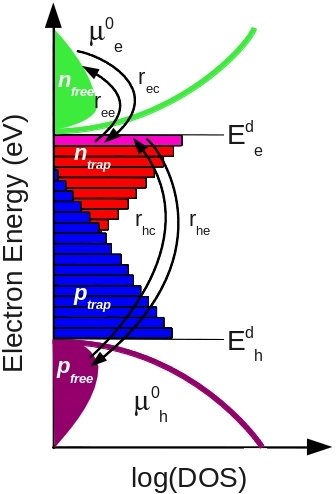
\includegraphics[width=40mm]{./images/dos_structure.jpg}
\caption{Trap filling in both energy and position space as the solar cell is taken from a negative bias
Carrier trapping, de-trapping, and recombination}
\label{fig:dos_structure}
\end{figure}

\begin{table}
\begin{center}
  \begin{tabular}{lll}
  \hline
  Mechanism & Symbol & Description  \\
  \hline
Electron capture rate & $r_{ec}$ & $n v_{th} \sigma_{n} N_{t}(1-f)$ \\
Electron escape rate & $r_{ee}$ & $e_{n} N_{t} f$ \\
Hole capture rate & $r_{hc}$ & $p v_{th} \sigma_{p} N_{t} f$ \\
Hole escape rate & $r_{he}$ & $e_{p} N_{t} (1-f)$\\
  \hline
\end{tabular}
\end{center}
\caption{Shockley-Read-Hall trap capture and emission rates, where $f$ is the fermi-Dirac occupation function and $N_{t}$ is the trap density of a single carrier trap.}
\label{tab:rates}
\end{table}



For each trap level the carrier balance \ref{eq:srhrate} is solved, giving each trap level an independent quasi-Fermi level. Each point in position space can be allocated between 10 and 160 independent trap states.  The rates of each process $r_{ec}$, $r_{ee}$, $r_{hc}$, and $r_{he}$ are give in table \ref{tab:rates}.

\begin{equation}
\label{eq:srhrate}
\frac{\delta n_t}{\partial t}=r_{ec}-r_{ee}-r_{hc}+r_{he}
\end{equation}

The escape probabilities are given by:

\begin{equation}
\label{eq:taile}
e_n=v_{th}\sigma_{n} N_{c} exp \left ( \frac{E_t-E_c}{kT}\right )
\end{equation}

and

\begin{equation}
\label{eq:taile}
e_p=v_{th}\sigma_{p} N_{v} exp \left ( \frac{E_v-E_t}{kT}\right )
\end{equation}

 where $\sigma_{n,p}$ are the trap cross sections, $v_{th}$ is the thermal emission velocity of the carriers, and $N_{c,v}$ are the effective density of states for free electrons or holes.  The distribution of trapped states (DoS) is defined between the mobility edges as

\begin{equation}
\label{eq:taile}
\rho^{e/h}(E)=N^{e/h}exp(E/E_{u}^{e/h})
\end{equation}

where , $N_{e/h}$ is the density of trap states at the LUMO or HOMO band edge
in states/eV and where $E_{U}^{e/h}$ is slope energy of the density of states. 

The value of $N_{t}$ for any given trap level is calculated by averaging the DoS function over the energy ($\Delta E$ ) which a trap occupies:

\begin{equation}
\label{eq:taile}
N_{t}(E)=\frac{\int^{E+\Delta E/2}_{E-\Delta E/2} \rho^{e}{E} dE}{\Delta E}
\end{equation}

The occupation function is given by the equation,
\begin{equation}
f(E_{t},F_{t})=\frac{1}{e^{\frac{E_{t}-F_{t}}{kT}}+1}
\end{equation}
Where, $E_{t}$ is the trap level, and $F_{t}$ is the Fermi-Level of the trap.
The carrier escape rates for electrons and holes are given by





\section{Free-to-free carrier recombination}
A free-carrier-to-free-carrier recombination (bi-molecular) pathway is also included.  Free-to-free recombination is described using equation \ref{equ:freetofree}

\begin{equation}
R_{free}=k_{r}(n_{f}p_{f}-n_{0}p_{0})
\label{equ:freetofree}
\end{equation}

in some situations where one is trying to fit rate equations to the model it can be useful to have equation \ref{equ:freetofree} written in another form,

\begin{equation}
R_{free}=k_{r}(n_{f}p_{f}-n_{0}p_{0})^{\frac{\lambda+1}{2}}
\label{equ:freetofree_lambda}
\end{equation}

this can be turned on using the option called  \emph{Enable $\lambda$ power in free to free recombination.} in the configure window of the Electrical parameter editor.

Free to free recombination is equivalent to Langevin recombination. However, most organic solar cells have a great deal of trap states and an ideality factor greater than 1.0 suggesting that free-to-free recombination is not the dominant mechanism. See section \ref{sec:the_need_for_trap_states} for a general discussion on the need for trap states and why generally Langevin recombination should not be used in organic solar device models. 

\section{Auger recombination}
\label{sec:auger}
Auger recombination is as

\begin{equation}
R^{AU}=(C^{AU}_{n}n+C^{AU}_{p}p)(np-n_{0}p_{0})
\end{equation}

where $C^{AU}_{n}$ and $C^{AU}_{p}$ are the Auger coefficient of electrons and holes in $m^6 s^{-1}$. This can be set in the electrical paramter editor.

%https://www.iue.tuwien.ac.at/phd/ayalew/node73.html

\section{Charge carrier transport}
To describe charge carrier transport, the bi-polar drift-diffusion equations are solved in position space
for electrons,
\begin{equation}
\label{eq:ndrive}
\boldsymbol{J_n} = q \mu_e n_{f}  {\nabla E_{c}}  + q D_n  {\nabla n_{f}},
\end{equation}
and holes,
\begin{equation}
\label{eq:pdrive}
\boldsymbol{J_p} = q \mu_h p_{f}  {\nabla E_{v}}  - q D_p {\nabla p_{f}}.
\end{equation}

Conservation of charge carriers is forced by solving the charge carrier continuity equations for both electrons,
\begin{equation}
\label{eq:contn}
\nabla \boldsymbol{J_n}  = q (R-G+\frac{\partial n}{\partial t}),
\end{equation}
and holes
\begin{equation}
\label{eq:contp}
\nabla \boldsymbol{J_p} = - q (R-G+\frac{\partial p}{\partial t}).
\end{equation}

where $R$ and $G$ are the net recombination and generation rates per unit volume respectively.

\section{Perovskite mobile ion solver}
The mobile ion solver is implemented after the work of Calado \cite{calado2016evidence}

\begin{equation}
\label{eq:pdrive}
\boldsymbol{J_a} = q \mu_a a_{f}  {\nabla E_{v}}  - q D_a {\nabla a_{f}}.
\end{equation}

\begin{equation}
\label{eq:contp}
\nabla \boldsymbol{J_a} = - q \frac{\partial a}{\partial t}.
\end{equation}



\section{Semiconductor interfaces}
The equations below came from section 4.16.3.1 "Possible Conduction Mechanisms" of in the chapter "Electronic Properties of Alkanethiol Molecular Junctions: Conduction Mechanisms, Metal–Molecule Contacts, and Inelastic Transport" in the book, Comprehensive Nanoscience and Technology. They are referenced to Sze SM (1981) Physics of Semiconductor Devices.
%But I can not see their table in Sze

\subsection{Direct tunnelling}
\begin{equation}
\boldsymbol{J} = A(n-n^{eq}) Vexp  \left( -\frac{2d}{\hbar} \sqrt{2m q\phi}  \right)
\end{equation}
$A$ is a constant, $V$ is the applied bias, and $\phi$ is the barrier height calculated from the band structure, m is the mass of an electron, and d is the thickness of the barrier. In the model this is implemented as:
\begin{equation}
\boldsymbol{J} = A(n-n^{eq}) Vexp  \left( -B \sqrt{\phi}  \right)
\end{equation}

\subsection{Tunnelling organic-organic}
This is not classical tunnelling, but assumes the carriers can drift into trap states at the interface, it is really only applicable for organics.

Tunnelling of holes through hetrojunction interfaces are is give by
\begin{equation}
\boldsymbol{J_p} = q T_{h}  ((p_{1}-p_{1}^{eq})-(p_{0}-p_{0}^{eq})),
\end{equation}

and for electrons

\begin{equation}
\boldsymbol{J_n} = -q T_{e}  ((n_{1}-n_{1}^{eq})-(n_{0}-n_{0}^{eq})).
\end{equation}

Where $T_{h}$ and $T_{e}$ represent the rate constants of the tunnelling. This can be configured in the interfaces editor.

%%%%%%%%%%%%%%%%%
\subsection{Fowler–Nordheim tunnelling}
\begin{equation}
\boldsymbol{J} = A(n-n^{eq}) V^2 exp  \left( -\frac{q4d\sqrt{2m} \phi^{3/2}}{3q \hbar V}  \right)
\end{equation}
\emph{Not yet implemented but could be on request.} $A$ is a constant, $V$ is the applied bias, and $\phi$ is the barrier height calculated from the band structure, m is the mass of an electron, and d is the thickness of the barrier.  In the model this is implemented as:

\begin{equation}
\boldsymbol{J} = A(n-n^{eq}) V^2 exp  \left( -\frac{B \phi^{3/2}}{V}  \right)
\end{equation}

\subsection{Thermionic emission}
\begin{equation}
\boldsymbol{J} = A(n-n^{eq}) T^2 exp  \left( -\frac{q\phi -q\sqrt{qV/ 4 \pi \epsilon d}}{kT}  \right)
\end{equation}

\emph{Not yet implemented but could be on request.} $A$ is a constant, $V$ is the applied bias, and $\phi$ is the barrier height calculated from the band structure, m is the mass of an electron, and d is the thickness of the barrier.  In the model this is implemented as:

\begin{equation}
\boldsymbol{J} = A(n-n^{eq}) T^2 exp  \left( -\frac{q\phi -B\sqrt{V}}{kT}  \right)
\end{equation}

\subsection{Hopping conduction}
\emph{Not yet implemented but could be on request.}
\begin{equation}
\boldsymbol{J} = A(n-n^{eq}) V exp  \left( -\frac{q\phi}{kT}  \right)
\end{equation}

\subsection{Doping on the interface}
Using the interface editor, layers of doping measuring one mesh point thick can be added to either side of the interface.  This is useful for OFET simulations where interface charge is important to the turn on voltage.


\newpage
\section{Configuring the electrical solver}
\label{sec:solverconfig}


Behind OghmaNano are a series of non-linear solvers that solve the electrical equations in a highly efficient way.  These can be configured by going to the electrical tab. There you will see the Drift diffusion button, to the left of that is an arrow. If you click on this it will bring up a window which allows you to configure the "Newton solver". The options are described below.

Related YouTube videos:
\begin{figure}[H]

\begin{tabular}{ c l }


\includegraphics[width=0.05\textwidth]{./images/youtube.png}

&
\href{https://www.youtube.com/watch?v=D2WG1_wTbdc}{How to optimize simulations in OghmaNano so they run faster}

\end{tabular}
\end{figure}

\begin{itemize}
  \item Max Electrical iterations (first step): The maximum number of steps the solver can after it's cold started onto a new problem.  This is usually at 0V in the dark.  The solver usually takes more steps on it's first go.
  \item Electrical clamp (first step): This is a number by which the maximum newton step is clamped to.  0.1 will make the solver very stable but very slow, 4.0 will make the solver very fast but unstable.  A recommended value of 1.0 is suggested for normal problems.  If you are solving for high doping or other unusual conditions it can be worth reducing the step.  Likewise if you want the solver to be fast and you know the problem is easy set the value to 2.0 or higher. For the first step, I would consider setting this value to be slightly lower than for the subsequent steps.
  \item Desired solver error (first step): This is the desired error, smaller is more accurate and slower. I would generally not accept answers above $1x10^{-5}$

  \item Max Electrical iterations: Maximum number of electrical iterations on all but the first step.
  \item Electrical clamp: Electrical clamp (first step): This is a number by which the maximum newton step is clamped to.  0.1 will make the solver very stable but very slow, 4.0 will make the solver very fast but unstable.  A recommended value of 1.0 is suggested for normal problems.  If you are solving for high doping or other unusual conditions it can be worth reducing the step.  Likewise if you want the solver to be fast and you know the problem is easy set the value to 2.0 or higher.
  \item Desired solver error: This is the desired error, smaller is more accurate and slower. I would generally not accept answers above $1x10^{-5}$

  \item Newton solver clever exit: If the solver starts bouncing in the noise then assume we can't get a better answer and quit.
  \item Newton minimum iterations: Don't allow the solver to quit before doing this number of steps.  Often the error in the first few steps of the solution can be below "Desired solver error", thus the solver can quit before finding the true answer.
  \item Solve Kirchhoff's current law in Newton solver: Solve Kirchhoff's current law in the main Newton Jacobian.

  \item Matrix solver:  This selects the matrix solver to use.
  \item Newton solver to use:
	\begin{itemize}
	  \item none: No electrical solver is selected, this is used when only solving optical or thermal problems.
	  \item newton: The standard 1D Newton solver.
	  \item newton\textunderscore 2D: The standard 2D Newton solver.
 	  \item newton\textunderscore norm: The standard 1D Newton solver but with Slotboom normalization.  This is handy when solving systems with large difference in density between minority and majority carrier density.
 	  \item poisson\textunderscore 2d: A 2D Poisson solver with no drift diffusion equations. 
	\end{itemize}
  \item Complex matrix solver:

  \item Slotboom T0: Slotboom variable for the newton\textunderscore norm solver.
  \item Slotboom D0: Slotboom variable for the newton\textunderscore norm solver.
  \item Slotboom n0: Slotboom variable for the newton\textunderscore norm solver.

  \item Use newton cache (experimental): Cache large problems to disk - experimental.
  \item Quit on convergence problem: Quit on convergence problem. Quite often 
  \item Quit on inverted Fermi-level:
  \item Solver output verbosity:

\end{itemize}

\subsection{Solver stability}
\label{sec:solverstability}

\subsubsection{Avoiding very big and very small numbers} \label{ssec:big_small_numbers}
Try opening up MATLAB (Octave if you are on Linux) and typing in the following equation $((1e-1+1e1)-1e1)/1e-1$. Before pressing enter, try to evaluate it in your head. the $1e1$ and the $-1e1$ cancel leaving $\frac{1e-1}{1e-1}$ which equates to $1$.  Now try replacing the powers to 1 with to the 19, so type in $((1e-19+1e19)-1e19)/1e-19$, again evaluate this in your head.  Again , $1e19$ and the $-1e19$ cancel leaving $\frac{1e-19}{1e-19}$ which equates to $1$  Now let the computer evaluate the expression.  In fact this time the computer does not give you $1$ but gives you $0$. Double check that you typed it in correctly... you did so what is happening. Why is the computer giving me an answer which is 100\% wrong.  The answer is easy, computers have a limited precision. This means that they can only store a limited number of decimal places. On a modern PC it's about 15 decimal places. After this the computer starts ignoring the numbers.  So when we added $(1e-19+1e19)$ the computer could not keep track of the decimal places so it assumed that the answer was exactly $1.000000000000000e19$ and not $1.0000000000000000001e19$, then when we subtracted $-1e19$ from the answer the computer gave us zero instead of $1e-19$.  The $1e-19$ was lost in the precision.

All computers are affected by this no matter how powerful they are, this has important implications when solving device equations.  If you have too big a spread of numbers in your simulation (matrix/Jacobian) the computer won't be able to solve it easily.  So if you have very low values of mobility say $1e-19$ and very big values say $1e5$ the computer wills start to have problems solving the electrical problem. There fore generally try to reduce the spread of parameters in you model. This is important when simulating insulators.

\subsubsection{Avoid zeros}
Zeros are bad because they cause divide by zero errors. So don't have zero mobilities, carrier cross sections, tail slopes or densities of states.  It's fine to have zero recombination constants though.

\subsubsection{Very big steps in the band gap}
Big steps in the band gap will produce very small and very large carrier densities - see \emph{Avoiding very big and very small numbers} above.


\newpage
\section{The need for trap states in device organic models}
\label{sec:the_need_for_trap_states}
Related YouTube videos:
\begin{figure}[H]

\begin{tabular}{ c l }


\includegraphics[width=0.05\textwidth]{./images/youtube.png}

&
\href{https://www.youtube.com/watch?v=2EHfulz7UDU}{Please stop simulating disordered semiconductors without trap states.}

\end{tabular}
\end{figure}
This section explains why trap states need to be considered when simulating disordered materials such as polymer/small molecule devices. It also touches on why using full SRH recombination/trapping model is so important to get physically meaningful results from a device model.

\subsection{The physical and energetic structure of disordered materials.}
Traditional inorganic semiconductor such as crystalline Si or GaAs are highly ordered and are almost completely pure it is not uncommon to get a material that is nine nines pure or, 99.9999999\% pure. Organic semiconductors on the other hand are very really quite dirty with purities often around 99.9\% which is six orders of magnitude more dirty than their inorganic counterparts, thus they have around a million times more impurities than their inorganic counterparts.  Added to this inorganic semiconductors are highly ordered with a regular crystalline structure one can think of them as marbles packed on a solitaire board (see Figure \ref{fig:order}), while organic semiconductors are a floppy mess of molecules which one can think of more as spaghetti bolognese with the spaghetti representing the polymers and the bolognese representing small molecules (see Figure \ref{fig:disorder}).

\begin{figure}[H]
\centering
\begin{tabular}{ c c }


\includegraphics[width=0.5\textwidth,height=0.4\textwidth]{./images/electrical/marbles.jpg}

&
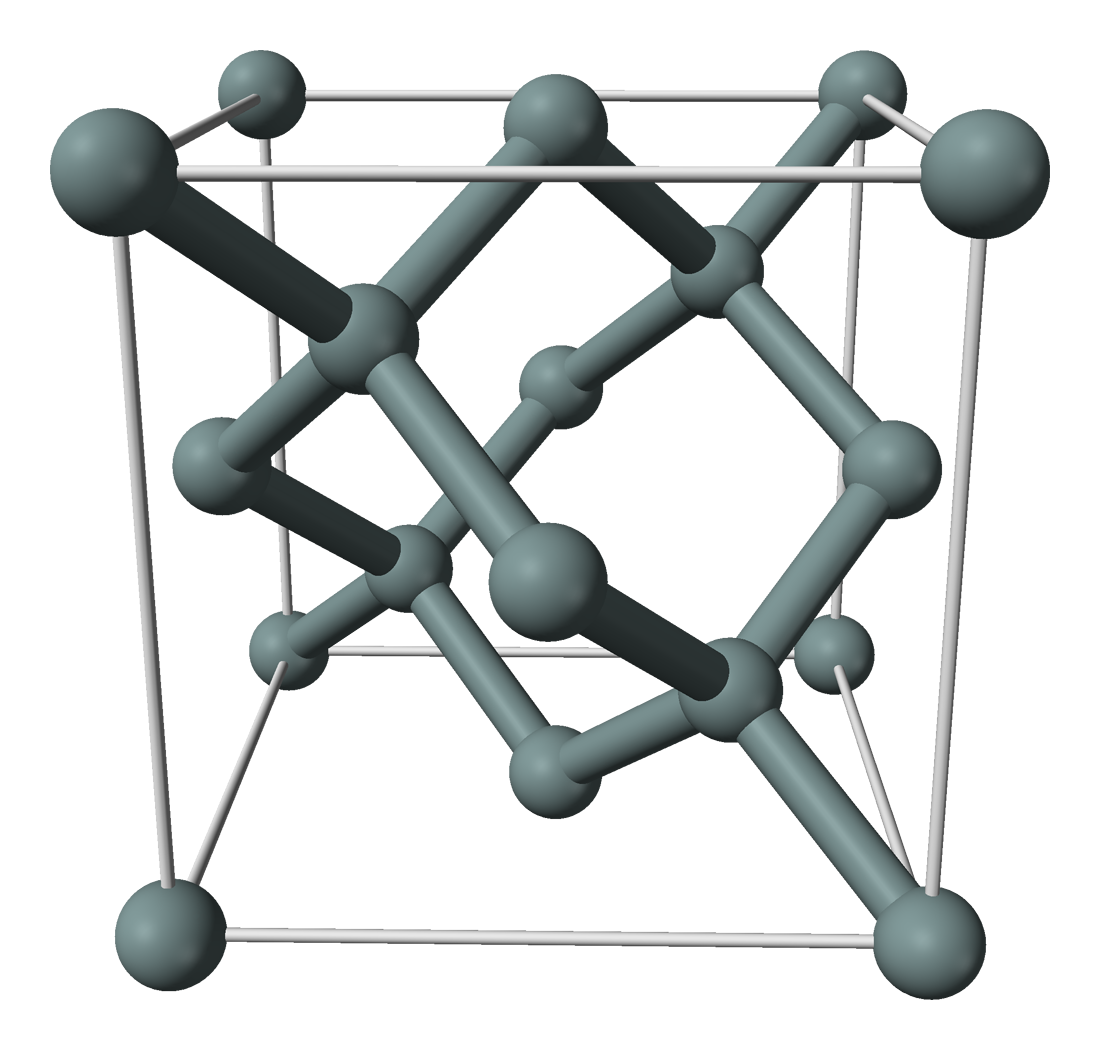
\includegraphics[width=0.5\textwidth,height=0.4\textwidth]{./images/electrical/silicon.png}
\\

\end{tabular}
\caption{Left) Marbles in an ordered arrangement on a solitaire board \cite{image_marbles}; Right) Silicon atoms ordered within a material\cite{image_silicon} Both systems are highly ordered.}
\label{fig:order}
\end{figure}

\begin{figure}[H]
\centering
\begin{tabular}{ c c }



\includegraphics[width=0.5\textwidth,height=0.4\textwidth]{./images/electrical/spaghetti.jpg}

&
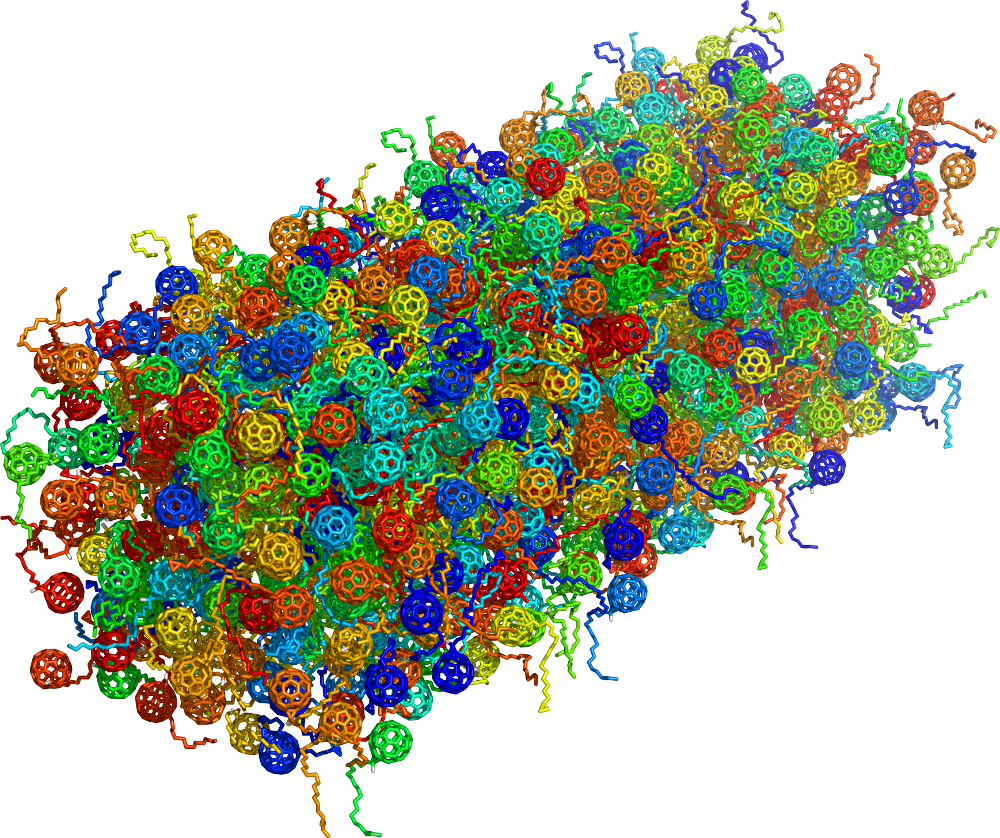
\includegraphics[width=0.5\textwidth,height=0.4\textwidth]{./images/electrical/polymer.png}
\\
\end{tabular}
\caption{Left) A plate of spaghetti \cite{image_spaghetti}; Right) A polymer packing like spaghetti. Both systems are highly disordered.}
\label{fig:disorder}
\end{figure}

So on one hand we have an organic material that is messy and highly disordered, and on the other hand we have a material such as silicon that is highly pure and very ordered.  This physical differences results in a very different energetic landscape for the two materials. In the ordered material semiconductor electrons/holes can travel freely in the conduction and valance bands. If an electric field is applied they only experience a small resistive force. Such a band structure is shown in Figure \ref{fig:band_structure}a. In the organic material the picture is very different, due to the disorder and impurities the band structure is full trap states. There are so many trap states that the carriers no longer move freely but hop between the trap states after being thermally excited, such a band structure is shown in shown in Figure \ref{fig:band_structure}b. Thus there are two very different charge transport mechanisms in these two materials.


\begin{figure}[H]
\centering
\begin{tabular}{ c c }


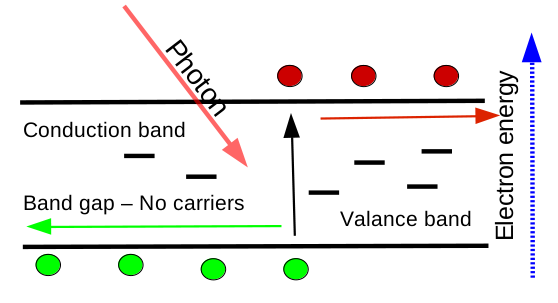
\includegraphics[width=0.5\textwidth,height=0.32\textwidth]{./images/electrical/ordered.png}

&
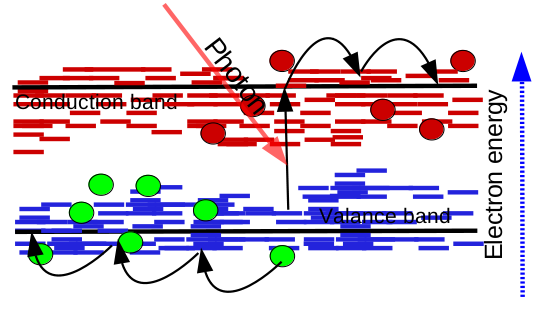
\includegraphics[width=0.5\textwidth,height=0.32\textwidth]{./images/electrical/disordered.png}
\\
\end{tabular}
\caption{a) The band structure of an ordered semiconductor such as GaAs; b) The band structure of an disordered material such as PM6:Y6 or P3HT:PCBM.}
\label{fig:band_structure}
\end{figure}

\subsection{Trap states and charge density}
[This section needs improving/editing but the sketch of what it should say is there:]
Figure \ref{fig:dos_image} sketches out the distribution of states for Figure \ref{fig:band_structure}. On the left of the image is a ordered semiconductor with a parabolic band structure. The Fermi distribution of electrons is coloured in purple. The right hand side image shows a disordered semiconductor with an exponential density of trap states going into the band gap (sometimes a Gaussian DoS is used).  It can be seen that the DoS and the distribution/energetic position of charge carriers are is very different between the two types of semiconductor.


\begin{figure}[H]
\centering
\begin{tabular}{ c c }

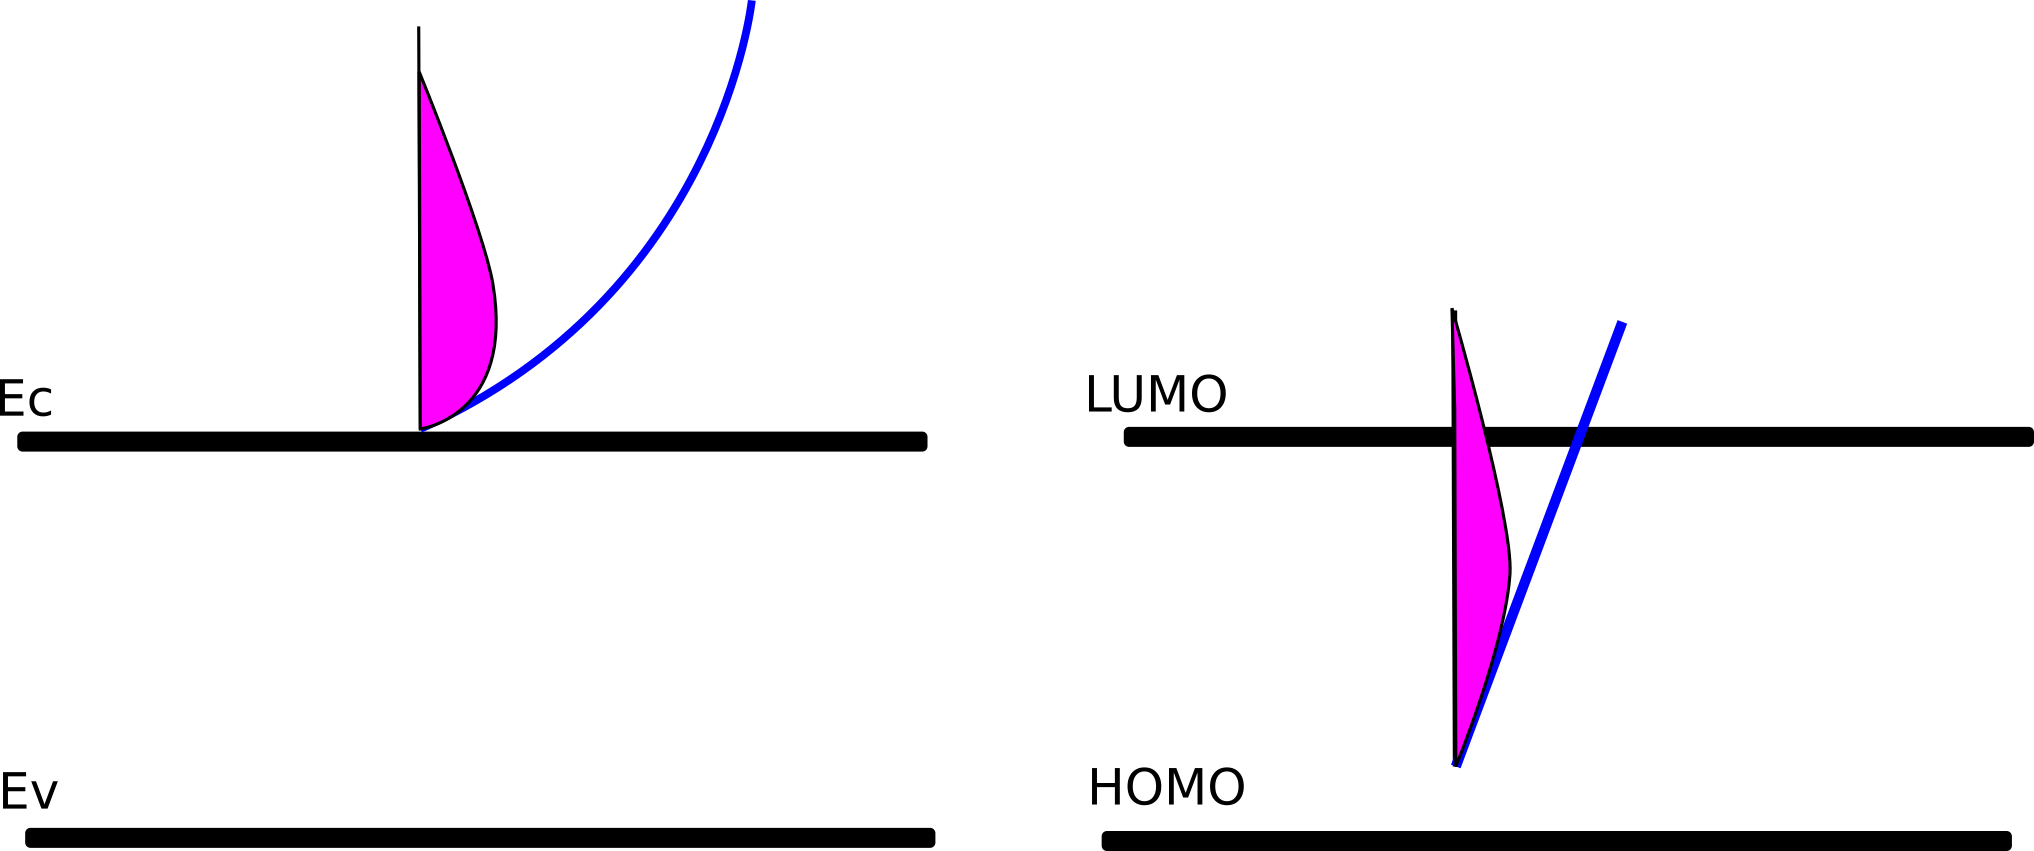
\includegraphics[width=1\textwidth,height=0.4\textwidth]{./images/electrical/band_structure.png}
\\
\end{tabular}
\caption{a) The band structure of an ordered semiconductor such as GaAs; b) The band structure of an disordered material such as PM6:Y6 or P3HT:PCBM.}
\label{fig:dos_image}
\end{figure}

The total charge density at any place in the device can be described by an integration of the Fermi-Dirac function, and the DoS $\rho$.

\begin{equation}
n(E_{f},T)=\int^{\infty}_{E_{min}} \rho(E) f(E,E_{f}) dE
\end{equation}

Where $E_{f}$ is the Fermi level. Clearly $\rho$ will be very different for an ordered and a disordered semiconductor. Thus the dependence of $n(E_{f},T)$ on $E_{f}$ and thus applied voltage will very depending on what $\rho$ is chosen for the device. In practical terms this means that a disordered device will have a lot more traps closer to the Fermi level and thus for any given voltage it will contain one or two orders of magnitude more charge than an ordered device, this can be observed in Charge Extraction experiments. So if one ignores trap states when modelling a disordered device then the function $n(Voltage)$ will be wrong.

If $n(Voltage)$ is not correct then the recombination rate will be wrong for any given voltage:

\begin{equation}
R=k_{r}n(Voltage) p(Voltage)
\end{equation}


Furthermore if $n_{free}(E_{f},T)$ is wrong the mobility will also have an incorrect dependence on voltage:

\begin{equation}
\mu_e(n)=\frac{\mu_e^0 n_{free}}{n_{free}+n_{trap}}
\end{equation}

So if your DoS is wrong (i.e. no traps). Then you have no chance of reproducing a JV curve correctly.  Summary: OghmaNano was written specifically to simulate disordered devices where trap states are play a large role in transport and recombination. Examples of such materials are PM6:Y6 and P3HT:PCBM. OghmaNano includes traps correctly, make sure what ever model you are using also includes traps or it will be wrong.

\subsection{Why you should not use Langevin recombination in device models}
Langevin recombination is defined as,

\begin{equation}
R_{free}=q k_{r}\frac{( \mu_e+ \mu_h) }{2\epsilon_0\epsilon_r} n p
\end{equation}

where $R_{free}$ is the recombination rate, $k_{r}$ is the Langevin reduction factor and all other symbols have their usual meaning. In general Langevin recombination is a bad way to describe recombination in OPV devices. There were some older papers from the early 2010s using this mechanisum but the models could not self consistently describe dark and light JV curves. This is because the mechanism assumes Brownian motion of electrons and holes and that charge carriers of opposite polarity will recombine when they get close enough to fall into each others electrostatic field.  This picture assumes the charge carriers are free and completely neglects the influence of trap states. It was often found that the Langevin equation could not reproduce the experimental results and predicted recombination rates far higher than were experimental observed. To account for this a Langevin reduction factor $k_{r}$ was often introduced into the equation, and a lot of effort went into measuring $k_{r}$. This need for a reduction factor pointed at some deeper issues with the equation.

If we look at the equation for Langevin recombination we can immediately see some issues with it. The first thing we notice is that $R_{free}$ can only ever change as the square of the charge density (n p), but we know from experiment $R_{free}$ can is often a higher order than 2 e.g. $(np)^{1.5}$. Furthermore we can see two mobility terms, however we know from the discussion from above that mobility is a function of carrier density. So the fact that it has the wrong dependence on carrier density and needs a reduction factor points at the mechanism on which it is based being incorrect, and using it will always be like trying to get a square peg in a round hole. 

\subsection{How one can make Langevin recombination work in device models}
So they key problems with Langevin recombination are a wrong dependence on carrier density and the need for a reduction factor. It is possible to make Langevin recombination 'work' by making the charge carrier mobilities a function of carrier density as was done in \cite{mackenzie2011modeling}:

\begin{equation}
R_{free}=q k_{r}\frac{(\alpha \mu_e(n)+\beta \mu_h(n)) n_{tot} p_{tot}}{2\epsilon_0\epsilon_r}
\end{equation}

then by defining a mobility edge and assuming any carrier below the mobility edge could not move and any carrier above it could.  One could define the averaged electron/hole mobility as: 

\begin{equation}
\mu_e(n)=\frac{\mu_e^0 n_{free}}{n_{free}+n_{trap}}
\end{equation}

and

\begin{equation}
\mu_h(n)=\frac{\mu_h^0 p_{free}}{p_{free}+p_{trap}}
\end{equation}

and if one assumes the density of free charge carriers is much smaller than the density of trapped charge carriers one can arrive at

\begin{equation}
R(n,p)=q k_{r}\frac{(\alpha \mu_e^0 n_{free} p_{trap}+\beta \mu_h p_{free} n_{trap}) }{2\epsilon_0\epsilon_r}
\end{equation}

Thus by making the mobility carrier density dependent we arrive at an expression for Langeving recombination that's dependent upon the density of free and trapped carriers (i.e. $n_{free} p_{trap}$ and $ p_{free} n_{trap}$). This is in principle the same as SRH recombination (i.e. a process involving free electrons (holes) recombining with trapped holes (electrons)).  This was a nice simple approach and it worked quite well in the steady state.  However, to make this all work we have to assume all electrons (holes) at any given position in space had a single quasi-Fermi level, which meant they were all in equilibrium with each other.  For this to be true, all electrons (holes) would have to be able to exchange energy with all other electrons (holes) at that position in space and have an infinite charge carrier thermalization velocity.  This is an OK assumption in steady state when electrons (holes) had time to exchange energy, however once we start thinking about things happening in time domain, it becomes harder to justify because there are so many trap states in the device it is unlikely that charge carriers will be able to act as one equilibrated gas with one quasi-Fermi level.  On the other hand the SRH mechanism does not make this assumption, so it is a better description of recombination/trapping.




\section{Calculating the built in potential}  \label{sssec:initial}
The first step to performing a device simulation, is to calculate the built in potential of the device.  To do this we must know the following things:

\begin{itemize}

  \item The majority carrier concentrations on the contacts $n$ and $p$.
  \item The effective densities of states $N_{LUMO}$ and $N_{HOMO}$.
  \item The effective band gap $E_g$

\end{itemize}

\begin{figure}[H]
\centering
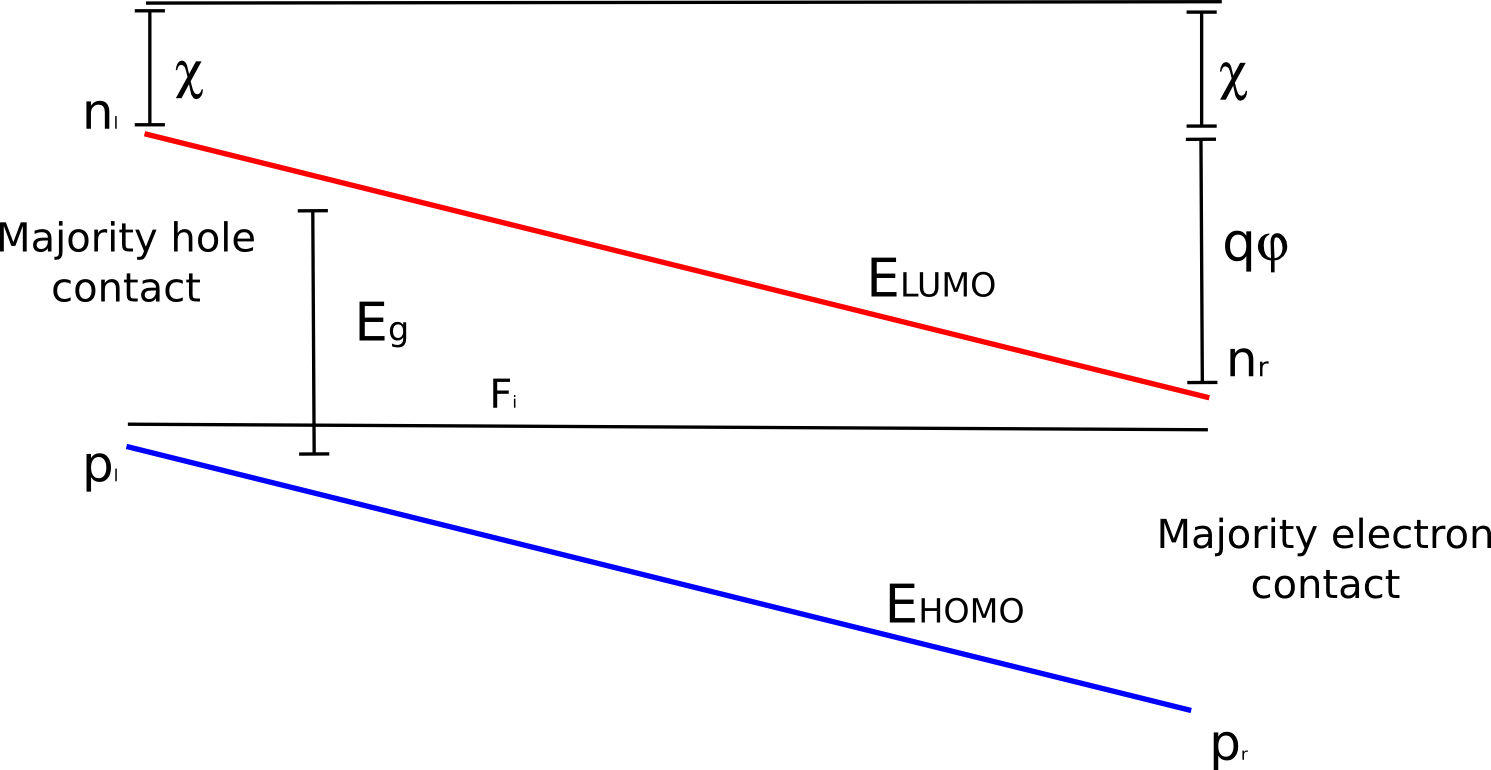
\includegraphics[width=120mm]{./images/bands.png}
\caption{Band structure of device in equilibrium.}
\label{fig:bands}
\end{figure}

\vspace{1em}
The left hand side of the device is given a reference potential of 0 V.  See figure \ref{fig:bands}.  We can then write the energy of the LUMO and HOMO on the left hand side of the device as:

\begin{equation}
E_{LUMO}=-\chi
\end{equation}

\begin{equation}
E_{HOMO}=-\chi-E_{g}
\end{equation}

For the left hand side of the device, we can use Maxwell-Boltzmann statistics to calculate the equilibrium Fermi-level ($F_i$).

\begin{equation}
p_{l}=N_v exp \left(\frac{E_{HOMO}-F_p}{kT} \right)
\end{equation}

We can then calculate the minority carrier concentration on the left hand side using $F_i$

\begin{equation}
n_{l}=N_c exp \left (\frac{F_n-E_{LUMO}}{kT} \right)
\end{equation}

The Fermi-level must be flat across the entire device because it is in equilibrium.  However we know there is a built in potential, we can therefore write the potential of the conduction and valance band on the right hand side of the device in terms of $phi$ to take account of the built in potential.

\begin{equation}
E_{LUMO}=-\chi-q\phi
\label{equ:Ev_rhs}
\end{equation}

\begin{equation}
E_{HOMO}=-\chi-E_g-q\phi
\end{equation}

we can now calculate the potential using

\begin{equation}
n_{r}=N_c exp \left (\frac{F_n-E_{LUMO}}{kT} \right)
\end{equation}
equation \ref{equ:Ev_rhs}.

The minority concentration on the right hand side can now also be calculated using.

\begin{equation}
p_{r}=N_v exp \left (\frac{E_v-F_{HOMO}}{kT} \right)
\end{equation}

The result of this calculation is that we now know the built in potential and minority carrier concentrations on both sides of the device.  Note, infinite recombination velocity on the contacts is assumed.  I have not included finite recombination velocities in the model simply because they would add four more fitting parameters and in my experience I have never needed to use them to fit any experimental data I have come across.

Once this calculation has been performed, we can estimate the potential profile between the left and right hand side of the device, using a linear approximation. From this the charge carrier densities across the device can be guessed.  The guess for potential and carrier densities, is then used to prime the main Newton solver.  Where the real value are calculated.  The Newton solver is described in the next section.



\subsection{Average free carrier mobility}
In this model there are two types of electrons (holes), free electrons (holes) and trapped electrons (holes).  Free electrons (holes) have a finite mobility of $\mu_e^0$ ($\mu_h^0$) and trapped electrons (holes) can not move at all and have a mobility of zero.  To calculate the average mobility we take the ratio of free to trapped carriers and multiply it by the free carrier mobility.:

\begin{equation}
\mu_e(n)=\frac{\mu_e^0 n_{free}}{n_{free}+n_{trap}}
\end{equation}

Thus if all carriers were free, the average mobility would be $\mu_e^0$ and if all carriers were trapped the average mobility would be 0.  It should be noted that only $\mu_e^0$ ($\mu_h^0$) are used in the model for computation and $\mu_e(n)$ is an output parameter.

The value of $\mu_e^0$ ($\mu_h^0$) is an input parameter to the model.  This can be edited in the electrical parameter editor.  The value of $\mu_e(n)$, and $\mu_h(p)$ are output parameters from the model.  The value of $\mu_e(n)$, and $\mu_h(p)$ change as a function of position, within the device, as the number of both free and trapped charge carriers change as a function of position.  The values of  $\mu_e(x)$, and $\mu_h(x)$ can be found in $mu\_n\_ft.dat$ and $mu\_p\_ft.dat$ within the $snapshots$ directory.  The spatially averaged value of mobility, as a function of time or voltage can be found in the files $dynamic\_mue.dat$ or $dynamic\_muh.dat$ within the dynamic directory.

Were one to try to measure mobility using a technique such as CELIV or ToF, one would expect to get a value closer to $\mu_e(n)$ or $\mu_h(p)$ rather than closer to $\mu_e^0$ or $\mu_h^0$.  It should be noted however, that measuring mobility in disordered materials is a difficult thing to do, and one will get a different experimental value of mobility depending upon which experimental measurement method one uses, furthermore, mobility will change depending upon the charge density profile within the device, and thus upon the applied voltage and light intensity.  To better understand this, try for example doing a CELIV simulation, and plotting $\mu_e(n)$ as a function of time (Voltage).  You will see that mobility reduces as the negative voltage ramp is applied, this is because carriers are being sucked out of the device.  Then try extracting the mobility from the transient using the CELIV equation for extracting mobility.  Firstly, the CELIV equation will give you one value of mobility, which is a simplification of reality as the value really changes during the application of the voltage ramp.  Secondly, the value you get from the equation will almost certainly not match either $\mu_e^0$ or any value of $\mu_e(n)$.  This simply highlights, the difficult of measuring $a$ value of mobility for a disordered semiconductor and that really when we quote a value of mobility for a disordered material, it really only makes sense to quote a value measured under the conditions a material will be used.  For example, for a solar cell, values of $\mu_e(n)$ and $\mu_h(n)$, would be most useful to know under 1 Sun at the $P_{max}$ point on a JV curve.

